13. \begin{figure}[ht!]
\center{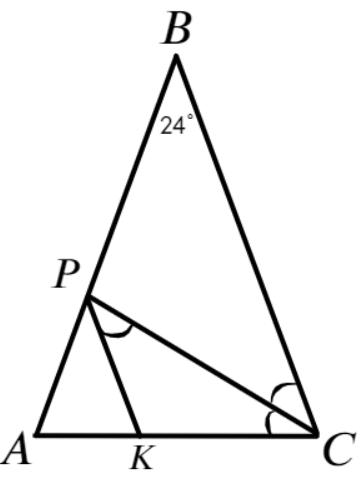
\includegraphics[scale=0.35]{g13.png}}
\end{figure}\\
Треугольник $ABC$ равнобедренный, поэтому $\angle C=(180^\circ-24^\circ):2=78^\circ.$ Так как $CP$ является биссектрисой, $\angle ACP=\angle BCP=78^\circ:2=39^\circ.$ Прямые $BC$ и $PK$ параллельны, $CP$ секущая, поэтому углы $KPC$ и $BCP$ равны как накрест лежащие, откуда $\angle KPC=39^\circ.$\\
